% \iffalse meta-comment
%
% Copyright (C) 2017--2021 by Xiangdong Zeng <xdzeng96@gmail.com>
%
% This work may be distributed and/or modified under the
% conditions of the LaTeX Project Public License, either
% version 1.3c of this license or (at your option) any later
% version. The latest version of this license is in:
%
%   http://www.latex-project.org/lppl.txt
%
% and version 1.3 or later is part of all distributions of
% LaTeX version 2005/12/01 or later.
%
% This work has the LPPL maintenance status `maintained'.
%
% The Current Maintainer of this work is Xiangdong Zeng.
%
% \fi

%*********************************************************************
% fduthesis: 复旦大学论文模板
% 2020/08/30 v0.7e
%
% 重要提示:
%   1. 请确保使用 UTF-8 编码保存
%   2. 请使用 XeLaTeX 或 LuaLaTeX 编译
%   3. 请仔细阅读用户文档
%   4. 修改、使用、发布本文档请务必遵循 LaTeX Project Public License
%   5. 不需要的注释可以尽情删除
%*********************************************************************

\documentclass{fduthesis}
% 模板选项:
%   type = doctor|master|bachelor  论文类型,默认为本科论文
%   oneside|twoside                论文的单双面模式,默认为 twoside
%   draft = true|false             是否开启草稿模式,默认关闭
% 带选项的用法示例:
%   \documentclass[oneside]{fduthesis}
%   \documentclass[twoside, draft=true]{fduthesis}
%   \documentclass[type=bachelor, twoside, draft=true]{fduthesis}

\fdusetup{
  % 参数设置
  % 允许采用两种方式设置选项:
  %   1. style/... = ...
  %   2. style = { ... = ... }
  % 注意事项:
  %   1. 不要出现空行
  %   2. “=” 两侧的空格会被忽略
  %   3. “/” 两侧的空格不会被忽略
  %   4. 请使用英文逗号 “,” 分隔选项
  %
  % style 类用于设置论文格式
  style = {
    % font = times,
    % 西文字体(包括数学字体)
    % 允许选项:
    %   font = garamond|libertinus|lm|palatino|times|times*|none
    %
    % cjk-font = fandol,
    % 中文字体
    % 允许选项:
    %   cjk-font = adobe|fandol|founder|mac|sinotype|sourcehan|windows|none
    %
    % 注意:
    %   1. 中文字体设置高度依赖于系统。各系统建议方案:
    %        windows:cjk-font = windows
    %        mac:    cjk-font = mac
    %        linux:  cjk-font = fandol(默认值)
    %   2. 除 fandol 和 sourcehan 外,其余字体均为商用字体,请注意版权问题
    %   3. 但 fandol 字体缺字比较严重,而 sourcehan 没有配备楷体和仿宋体
    %   4. 这里中西文字体设置均注释掉了,即使用默认设置:
    %        font     = times
    %        cjk-font = fandol
    %   5. 使用 font = none / cjk-font = none 关闭默认字体设置,需手动进行配置
    %
    font-size = 5,
    % 字号
    % 允许选项:
    %   font-size = -4|5
    %
    % fullwidth-stop = catcode,
    % 是否把全角实心句点 “.” 作为默认的句号形状
    % 允许选项:
    %   fullwidth-stop = catcode|mapping|false
    % 说明:
    %   catcode   显式的 “。” 会被替换为 “.”(e.g. 不包括用宏定义保存的 “。”)
    %   mapping   所有的 “。” 会被替换为 “.”(使用 LuaLaTeX 编译则无效)
    %   false     不进行替换
    %
    footnote-style = xits,
    % 脚注编号样式
    % 允许选项:
    %   footnote-style = plain|libertinus|libertinus*|libertinus-sans|
    %                    pifont|pifont*|pifont-sans|pifont-sans*|
    %                    xits|xits-sans|xits-sans*
    %
    % hyperlink = color,
    % 超链接样式
    % 允许选项:
    %   hyperlink = border|color|none
    %
    % hyperlink-color = default,
    % 超链接颜色
    % 允许选项:
    %   hyperlink-color = default|classic|elegant|fantasy|material|
    %                     business|science|summer|autumn|graylevel|prl
    % 默认与西文字体保持一致
    %
    bib-backend = bibtex,
    % 参考文献支持方式
    % 允许选项:
    %   bib-backend = bibtex|biblatex
    %
    % bib-style = numerical,
    % 参考文献样式
    % 允许选项:
    %   bib-style = author-year|numerical|<其他样式>
    % 说明:
    %   author-year  著者—出版年制
    %   numerical    顺序编码制
    %   <其他样式>   使用其他 .bst(bibtex)或 .bbx(biblatex)格式文件
    %
    % cite-style = {},
    % 引用样式
    % 默认为空,即与参考文献样式保持一致
    % 仅适用于 biblatex;如要填写,需保证相应的 .cbx 格式文件能被调用
    %
    bib-resource = {fduthesis-template.bib},
    % 参考文献数据源
    % 可以是单个文件,也可以是用英文逗号 “,” 隔开的一组文件
    % 如果使用 biblatex,则必须明确给出 .bib 后缀名
    %
    % logo = {fudan-name.pdf},
    % 封面中的校名图片
    % 模版已自带,通常不需要额外配置
    %
    % logo-size = {0.5\textwidth},      % 只设置宽度
    % logo-size = {{}, 3cm},            % 只设置高度
    % logo-size = {8cm, 3cm},           % 设置宽度和高度
    % 设置校名图片的大小
    % 通常不需要调整
    %
    % auto-make-cover = true
    % 是否自动生成论文封面(封一)、指导小组成员名单(封二)和声明页(封三)
    % 除非特殊需要(e.g. 不要封面),否则不建议设为 false
  },
  %
  % info 类用于录入论文信息
  info = {
    title = {论文标题},
    % 中文标题
    % 长标题建议使用 “\\” 命令手动换行(不是指在源文件里输入回车符,当然
    % 源文件里适当的换行可以有助于代码清晰):
    %   title = {最高人民法院、最高人民检察院关于适用\\
    %            犯罪嫌疑人、被告人逃匿、死亡案件违法所得\\
    %            没收程序若干问题的规定},
    %
    title* = {Thesis Title},
    % 英文标题
    %
    author = {王二},
    % 作者姓名
    %
    % author* = {Your name},
    % 作者姓名(英文 / 拼音)
    % 目前不需要填写
    %
    supervisor = {某某某\quad 教授},
    % 导师
    % 姓名与职称之间可以用 \quad 打印一个空格
    %
    major = {物理学},
    % 专业
    %
    degree = academic,
    % 学位类型
    % 允许选项:
    %   degree = academic|professional
    % 说明:
    %   academic      学术学位
    %   professional  专业学位
    %
    department = {物理系},
    % 院系
    %
    student-id = {12300000000},
    % 作者学号
    %
    % date = {2021 年 1 月 1 日},
    % 日期
    % 注释掉表示使用编译日期
    %
    % secret-level = ii,
    % 密级
    % 允许选项:
    %   secret-level = none|i|ii|iii
    % 说明:
    %   none  不显示密级与保密年限
    %   i     秘密
    %   ii    机密
    %   iii   绝密
    %
    % secret-year = {五年},
    % 保密年限
    % secret-level = none 时该选项无效
    %
    instructors = {
      {张\quad 三 \quad 教\quad 授},
      {李\quad 四 \quad 教\quad 授},
      {王五六     \quad 研究员}
    },
    % 指导小组成员
    % 使用英文逗号 “,” 分隔
    % 如有需要,可以用 \quad 手工对齐
    %
    keywords = {不确定关系, 量子力学, 理论物理},
    % 中文关键字
    % 使用英文逗号 “,” 分隔
    %
    keywords* = {Uncertainty principle, quantum mechanics, theoretical physics},
    % 英文关键字
    % 使用英文逗号 “,” 分隔
    %
    clc = {O413.1}
    % 中图分类号
  }
}

% 需要的宏包可以自行调用
\usepackage{physics}

% 需要的命令可以自行定义
\newcommand{\hilbertH}{\symcal{H}}
\newcommand{\ee}{\symrm{e}}
\newcommand{\ii}{\symrm{i}}

\begin{document}

% 这个命令用来关闭版心底部强制对齐,可以减少不必要的 underfull \vbox 提示,但会影响排版效果
% \raggedbottom

% 前置部分包含目录、中英文摘要以及符号表等
\frontmatter

% 目录
\tableofcontents
% 插图目录
\listoffigures
% 表格目录
% \listoftables

\begin{abstract}
  中文摘要
\end{abstract}

\begin{abstract*}
  English abstract
\end{abstract*}

% 符号表
% 语法与 LaTeX 表格一致:列用 & 区分,行用 \\ 区分
% 如需修改格式,可以使用可选参数:
%   \begin{notation}[ll]
%     $x$ & 坐标 \\
%     $p$ & 动量
%   \end{notation}
% 可选参数与 LaTeX 标准表格的列格式说明语法一致
% 这里的 “ll” 表示两列均为自动宽度,并且左对齐
\begin{notation}[ll]
  $x$                  & 坐标        \\
  $p$                  & 动量        \\
  $\psi(x)$            & 波函数      \\
  $\bra{x}$            & 左矢(bra) \\
  $\ket{x}$            & 右矢(ket) \\
  $\ip{\alpha}{\beta}$ & 内积        \\
\end{notation}

% 主体部分是论文的核心
\mainmatter

% 建议采用多文件编译的方式
% 比较好的做法是把每一章放进一个单独的 tex 文件里,并在这里用 \include 导入,例如
%   \include{chapter1}
%   \include{chapter2}
%   \include{chapter3}

\chapter{介绍}

\strong{量子力学}是物理学的分支学科。它主要描写微观的事物,与相对论一起被认为是现代物理学的两大
基本支柱,许多物理学理论和科学,如原子物理学、固体物理学、核物理学和粒子物理学以及其它相关的学科,
都是以其为基础\cite{曾谨言2013量子力学,feynman2011feynman}。

\section{量子力学历史概要}

\section{研究对象}

\section{研究方法}

\chapter{数学基础}

\section{基础公设}

整个量子力学的数学理论可以建立于五个基础公设。这些公设不能被严格推导出来的,而是从实验结果仔细分析
归纳总结而得到的。从这五个公设,可以推导出整个量子力学。假若量子力学的理论结果不符合实验结果,
则必须将这些基础公设加以修改,直到没有任何不符合之处。至今为止,量子力学已被实验核对至极高准确度,
还没有找到任何与理论不符合的实验结果,虽然有些理论很难直觉地用经典物理的概念来理解,例如,波粒
二象性、量子纠缠等等\cite{zurek2014quantum,cohen2013claude,zettili2003quantum}。

\begin{enumerate}
  \item 量子态公设:量子系统在任意时刻的状态(量子态)可以由希尔伯特空间 $\hilbertH$ 中的态矢量
    $\ket{\psi}$ 来设定,这态矢量完备地给出了这量子系统的所有信息。这公设意味着量子系统遵守%
    \emph{态叠加原理},假若 $\ket*{\psi_1}$、$\ket*{\psi_2}$ 属于希尔伯特空间 $\hilbertH$,则
    $c_1\ket*{\psi_1} + c_2\ket*{\psi_2}$ 也属于希尔伯特空间 $\hilbertH$。
  \item 时间演化公设: 态矢量为 $\ket{\psi(t)}$ 的量子系统,其动力学演化可以用薛定谔方程表示:
    \begin{equation}
      \ii\hbar \pdv{t} \ket{\psi(t)} = \hat{H} \ket{\psi(t)}.
    \end{equation}
    其中,哈密顿算符 $\hat{H}$ 对应于量子系统的总能量,$\hbar$ 是约化普朗克常数。根据薛定谔方程,
    假设时间从 $t_0$ 变化到 $t$,则态矢量从 $\ket*{\psi(t_0)}$ 演化到 $\ket{\psi(t)}$,该过程以
    方程表示为
    \begin{equation}
      \ket{\psi(t)} = \hat{U}(t,\,t_0) \ket*{\psi(t_0)}.
    \end{equation}
    其中 $\hat{U}(t,\,t_0) = \ee^{-\ii\hat{H}(t-t_0) / \hbar}$ 是时间演化算符。
  \item 可观察量公设:每个可观察量 $A$ 都有其对应的厄米算符 $\hat{A}$,而算符 $\hat{A}$ 的所有
    本征矢量共同组成一个完备基底。
  \item 坍缩公设:对于量子系统测量某个可观察量 $A$ 的过程,可以数学表示为将对应的厄米算符
    $\hat{A}$ 作用于量子系统的态矢量 $\ket{\psi}$,测量值只能为厄米算符 $\hat{A}$ 的本征值。
    在测量后,假设测量值为 $a_i$,则量子系统的量子态立刻会坍缩为对应于本征值 $a_i$ 的本征态
    $\ket*{e_i}$。
  \item 波恩公设:对于这测量,获得本征值 $a_i$ 的概率为量子态 $\ket{\psi}$ 处于本征态 $\ket*{e_i}$
    的概率幅的绝对值平方。\footnote{%
      使用可观察量 $A$ 的基底 $\qty{e_1,\,e_2,\,\ldots,\,e_n}$,量子态 $\ket{\psi}$ 可以表示为
      $\ket{\psi} = \sum_j c_j \ket*{e_j}$,其中 $c_j$ 是量子态 $\ket{\psi}$ 处于本征态
      $\ket*{e_j}$ 的概率幅。根据波恩定则,对于此次测量,获得本征值 $a_i$ 的概率为
      $\abs*{\ip*{e_i}{\psi}}^2 = \abs*{c_i}^2$。}
\end{enumerate}

\section{量子态与量子算符}

量子态指的是量子系统的状态,态矢量可以用来抽象地表现量子态。采用狄拉克标记,态矢量表示为右矢
$\ket{\psi}$;其中,在符号内部的希腊字母 $\psi$ 可以是任何符号、字母、数字,或单字。例如,
沿着磁场方向测量电子的自旋,得到的结果可以是上旋或是下旋,分别标记为 $\ket{\uparrow}$ 和
$\ket{\downarrow}$。

\begin{figure}[htb]
  \centering
  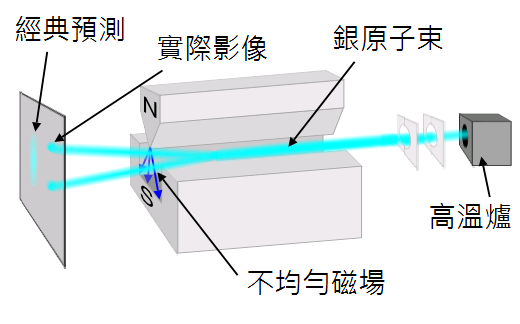
\includegraphics[width=0.5\textwidth]{fduthesis-template-image.png}
  \caption[施特恩—格拉赫实验]{%
    设定施特恩—格拉赫实验仪器的磁场方向为 $z$-轴,入射的银原子束可以被分裂成两道银原子束,每一道
    银原子束代表一种量子态,上旋 $\ket{\uparrow}$ 或下旋 $\ket{\downarrow}$%
    \cite{wikimedia:stern-gerlach-experiment}。}
  \label{fig:stern-gerlach-experiment}
\end{figure}

对量子态做操作定义,量子态可以从一系列制备程序来辨认,即这程序所制成的量子系统拥有这量子态。例如,
使用施特恩—格拉赫实验仪器,设定磁场朝着 $z$-轴方向,如图~\ref{fig:stern-gerlach-experiment} 所示,
可以将入射的银原子束,依照自旋的 $z$-分量分裂成两道,一道为上旋,量子态为 $\ket{\uparrow}$;另一道
为下旋,量子态为 $\ket{\downarrow}$,这样,可以制备成量子态为 $\ket{\uparrow}$ 的银原子束,或量子态
为 $\ket{\downarrow}$ 的银原子束。原本银原子束的态矢量可以按照态叠加原理表示为
\begin{equation}
  \ket{\psi} = \alpha \ket{\uparrow} + \beta \ket{\downarrow}.
\end{equation}
其中,$\alpha$、$\beta$ 是复值系数,$\abs{\alpha}^2$、$\abs{\beta}^2$ 分别为入射银原子束处于上旋、
下旋的概率,且有
\begin{equation}
  \abs{\alpha}^2 + \abs{\beta}^2 = 1.
\end{equation}

\section{动力学演化}

\chapter{总结与展望}

% 后置部分包含参考文献、声明页(自动生成)等
\backmatter

% 打印参考文献列表
\printbibliography

\end{document}
